\newpage
\subsection*{\textbf{Задание для самостоятельной работы}}

\begin{enumerate}
    \item Разложите на множители и на слагаемые выражение
    \[\sin[x]^2 \cos[x]^2+4 \sin[x] \cos[x]+1,\]
    используя материал \textnumero8 по символьным преобразованиям, воспользуйтесь панелью Algebraic Manipulation;
    \begin{figure}[H]
        \renewcommand{\figurename}{Рисунок}
        \centering{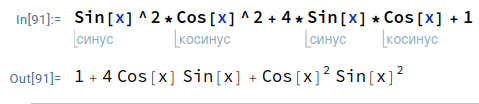
\includegraphics[scale=0.70]{body/img/self_1_1.png}}
        \label{fig:image_self_1_1}
    \end{figure}
    \item вычислите пределы следующих функций: \\
    $\ln(2x+1)-\ln(x+2)$, при  $x\to\infty$ \\
    а также $\frac{e^{ax}-e^{bx}}{x}$ при $x\to0$;
    \begin{figure}[H]
        \renewcommand{\figurename}{Рисунок}
        \centering{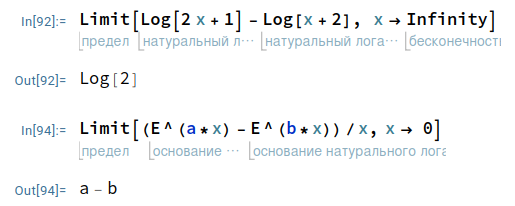
\includegraphics[scale=0.70]{body/img/self_1_2.png}}
        \label{fig:image_self_1_2}
    \end{figure}
    \item вычислите производную функцию
    \[f(x) = -\frac{1}{4(x^2+a^2)^2};\]
    \begin{figure}[H]
        \renewcommand{\figurename}{Рисунок}
        \centering{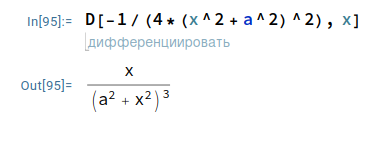
\includegraphics[scale=0.70]{body/img/self_1_3.png}}
        \label{fig:image_self_1_3}
    \end{figure}
    \item найдите неопределённый интеграл
    \[ \int\frac{x}{a+ bx}dx; \]
    \begin{figure}[H]
        \renewcommand{\figurename}{Рисунок}
        \centering{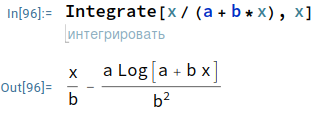
\includegraphics[scale=0.70]{body/img/self_1_4.png}}
        \label{fig:image_self_1_4}
    \end{figure}
    \item найдите определённый интеграл при $x$ от $a$ до $b$ в символьном виде, перед началом вычисления очистите значение
    параметров $a$ и $b$ с помощью оператора Clear:
    \[ \int_{a}^b\frac{x^2}{(a+bx)^2}dx. \]
    \begin{figure}[H]
        \renewcommand{\figurename}{Рисунок}
        \centering{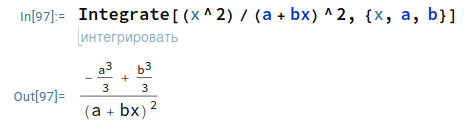
\includegraphics[scale=0.70]{body/img/self_1_5.png}}
        \label{fig:image_self_1_5}
    \end{figure}
    \item Создайте единичную матрицу $5\times5$ с использованием специальной функции.
    Задайте матрицу $5\times5$ с произвольными элементами, вычислите произведение созданных матриц.
    \begin{figure}[H]
        \renewcommand{\figurename}{Рисунок}
        \centering{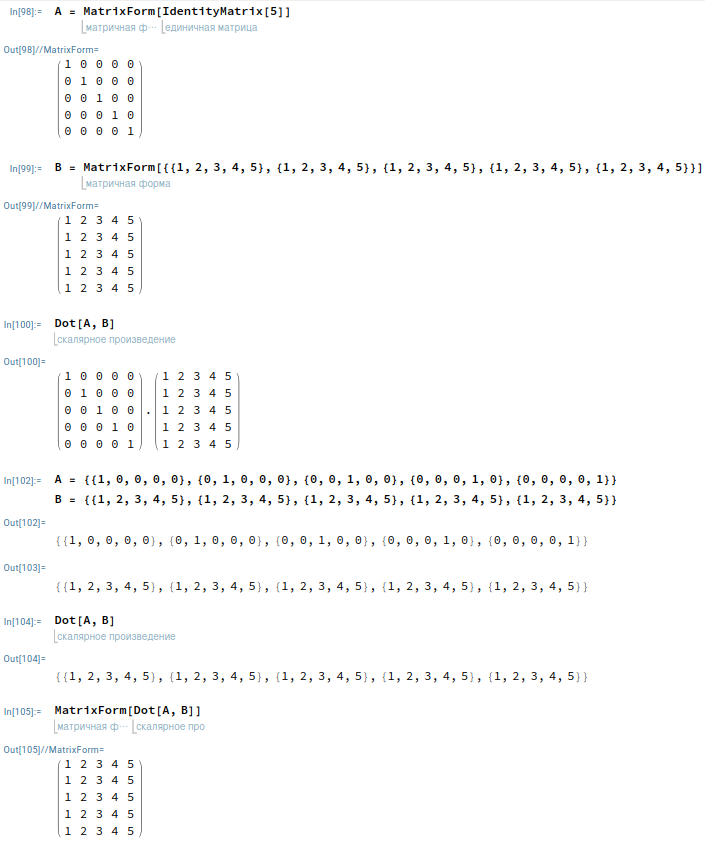
\includegraphics[scale=0.70]{body/img/self_1_6.png}}
        \label{fig:image_self_1_6}
    \end{figure}
\end{enumerate}